\chapter{Eksperyment zerowy}\label{chap:experiment_zero}

Po przygotowaniu komponentów systemu wstępnie zaimplementowano program rozwiązujący problem multilateracji, aby zbadać czy problem nie jest zbyt trywialny, aby opisać go w pracy, lub przeciwnym razie, na podstawie wyników eksperymentu, zastanowić się jakie przeszkody stoją na drodze do rozwiązania o zadowalającej precyzji.

\section{Opis działania}

Programy dla urządzeń w systemie zaimplementowano na podstawie rozwiązania aproksymacyjnego \ref{eq:lls} postaci
\begin{equation}
    \hat{\mathbf{x}} = {\left(\mathbf{A}^T\mathbf{A}\right)}^{-1}\mathbf{A}^T\mathbf{b}
\end{equation}
Poniżej przedstawiono je w formie pseudokodów. Współrzędne odbiorników, a zatem macierz $\mathbf{A}$ są znane i stałe dla każdej konfiguracji ustawienia odbiorników.

\subsection{Programy węzłów}

\begin{center}
    \captionof{algorithm}{Program nadajnika}\label{alg:source}
    \begin{algorithmic}[1]
        \State\ $buzz \gets False$
        \State\ $buzzTime \gets 0$
        \State\ $lastBuzzTime \gets 0$
        \State\ $syncTime \gets 0$

        \Function{onMessage}{$message, topic$}
            \If{$topic$ is $TOPIC$}
                \State\ $buzz \gets message$
            \EndIf
            \If{$topic$ is $TIME\_TOPIC$}
                \State\ $syncTime \gets micros()$
            \EndIf
        \EndFunction

        \Loop
            \If{$buzz$ and $micros() - lastBuzzTime > BUZZ\_INTERVAL$}
                \State\ $buzzTime \gets micros() - syncTime$
                \State\ $publish(buzzTime)$
                \State\ $lastBuzzTime \gets buzzTime$
                \State\ $buzzer()$
            \EndIf
        \EndLoop
    \end{algorithmic}
    \vspace{5pt}
    \hrule
\end{center}
%\newpage
\begin{center}
    \captionof{algorithm}{Program odbiornika}\label{alg:sink}
    \begin{algorithmic}[1]
        \State\ $micState \gets LOW$
        \State\ $micTime \gets False$
        \State\ $lastMicTime \gets 0$
        \State\ $syncTime \gets 0$

        \Function{onMessage}{$topic$}
            \If{$topic$ is $TIME\_TOPIC$}
                \State\ $syncTime \gets micros()$
            \EndIf
        \EndFunction

        \Function{micInterrupt}{}
            \State\ $micState \gets HIGH$
        \EndFunction

        \Loop
            \If{$micState$ is $HIGH$ and $micros() - lastMicTime > MIC\_INTERVAL$}
                \State\ $micTime \gets micros() - syncTime$
                \State\ $publish(micTime)$
                \State\ $lastMicTime \gets micTime$
                \State\ $micState \gets LOW$
            \EndIf
        \EndLoop
    \end{algorithmic}
    \vspace{5pt}
    \hrule
\end{center}

\begin{itemize}
    \item $micros()$ {-} funkcja zwracająca liczbę mikrosekund od uruchomienia urządzenia,
    \item $buzzer()$ {-} funkcja nadająca sygnał dźwiękowy przy użyciu brzęczyka,
    \item $TOPIC$ {-} nazwa kanału MQTT korespondującego do danego węzła,
    \item $TIME\_TOPIC$ {-} nazwa ogólnego kanału MQTT służącego do przesyłania wiadomości z poleceniem synchronizacji czasu,
    \item $BUZZ\_INTERVAL$ {-} interwał czasowy pomiędzy sygnałami brzęczyka,
    \item $MIC\_INTERVAL$ {-} interwał czasowy pomiędzy dwoma oddzielnymi rejestracjami wysokiego poziomu sygnału na mikrofonie,
    \item \textsc{onMessage} {-} funkcja wywołania zwrotnego wywoływana przy otrzymaniu wiadomości na dowolnym z subskrybowanych tematów,
    \item $publish()$ {-} funkcja publikująca wiadomość na zadanym kanale MQTT.
\end{itemize}

W celu zminimalizowania opóźnień funkcja \textsc{micInterrupt} została zaimplementowana przy użyciu przerwania sprzętowego. Jest wywoływana przy zmianie stanu pinu, do którego podłączony jest mikrofon z niskiego na wysoki.

\subsection{Program serwera}

\begin{center}
    \captionof{algorithm}{Program serwera}\label{alg:server}
    \begin{algorithmic}[1]
        \State\ $M \gets {\left(A^T A\right)}^{-1} A^T$
        \Function{$calc\_position$}{}
            \For{$node$ in $NODES$}
                \State\ $d \gets (SS / 10^{6}) \cdot time_{node} - time_{source}$
                \State\ $b_{node} \gets d - \sum_{x \in coords_{node}}{x^2}$
            \EndFor
            \State\ return $M \cdot b$
        \EndFunction
        \Loop{ $main$}
            \State\ $sleep(t_1)$
            \State\ $calc\_position()$
        \EndLoop
        \Loop{ $sync\_clock$}{}
            \State\ $publish(TIME\_TOPIC)$
            \State\ $sleep(t_2)$
        \EndLoop
    \end{algorithmic}
    \vspace{5pt}
    \hrule
\end{center}

\begin{itemize}
    \item $A$ - macierz zawierająca współrzędne obiorników z równania \ref{eq:matrix}
    \item $SS$ {-} prędkość dźwięku $\left[\frac{m}{s}\right]$,
    \item $time$ {-} czas dostarczony w ostatniej wiadomości od węzła,
    \item $coords$ {-} współrzędne węzłów nadawczych,
    \item $t_1$ {-} czas pomiędzy obliczeniami pozycji,
    \item $t_2$ {-} czas pomiędzy wiadomościami synchronizującymi zegary.
\end{itemize}

\subsection{Opis algorytmu}

W programie serwera zaimplementowano funkcję rozwiązującą równanie~\ref{eq:lls} przy pomocy funkcji bibliotecznych dostępnych w pakiecie \texttt{numpy}. Wywołania następują co interwał $t_1$. Co interwał $t_2$ serwer wysyła wiadomość synchronizującą z założeniem, że węzły odbierają ją równocześnie i w ten sposób synchronizują zegary.

\section{Ewaluacja działania systemu}

Pierwsze testy przeprowadzone zostały na systemie operującym w jednym wymiarze (to jest wszystkie węzły są współliniowe) w celu jak największego uproszczenia, pozwalającego na szybsze wykrywanie i rektyfikację błędów. Wszystkie odległości będą podawane w metrach.

\subsection{Struktura systemu testowego}

\begin{figure}[h]
    \centering
    \begin{tikzpicture}[pointnode/.style={circle, fill=black}, node distance=5cm, minimum size=5mm]
        \node[pointnode,
              label=above:{Nadajnik},
              label=below:{$0$}] (N) {};
        \node[pointnode,
              label=above:{Odbiornik 1.},
              label=below:{$-0.5$}] (O1) [left=of N] {};
        \node[pointnode,
              label=above:{Odbiornik 2.},
              label=below:{$0.5$}] (O2) [right=of N] {};
        \draw[-, thin, dotted] (-8,0) -- (8,0);
    \end{tikzpicture}
    \caption{Układ systemu testowego}
    \label{fig:test_setup}
\end{figure}

Nadajnik umiejscowiono w punkcie $(0)$, natomiast dwa odbiorniki w punktach odpowiednio $(-0.5)$ i $(0.5)$, wszystkie węzły były stacjonarne. Nadajnik co $0.5$ $s$ nadawał sygnał o długości $10$ $ms$, a serwer co $0.5$ $s$ zwracał wynik zagadnienia multilateracji na podstawie ostatnio otrzymanych danych. Wykonano 5 następujących bezpośrednio po sobie eksprymentów, poniżej przedstawiono wyniki trzech pierwszych, ponieważ są wystarczające do ukazania zachodzącego trendu.

\begin{figure}[H]
    \centering
    \begin{subfigure}{\textwidth}\label{fig:position_0}
        \centering
        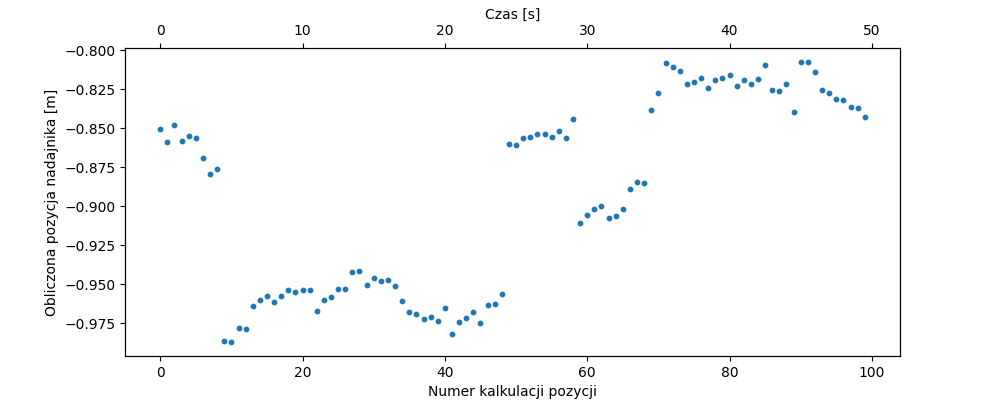
\includegraphics[width=\linewidth]{pics/position/position_0.png}
        \caption{Test 1.}
    \end{subfigure}
\end{figure}
\begin{figure}[H]
    \ContinuedFloat\centering
    \begin{subfigure}{\textwidth}\label{fig:position_1}
        \centering
        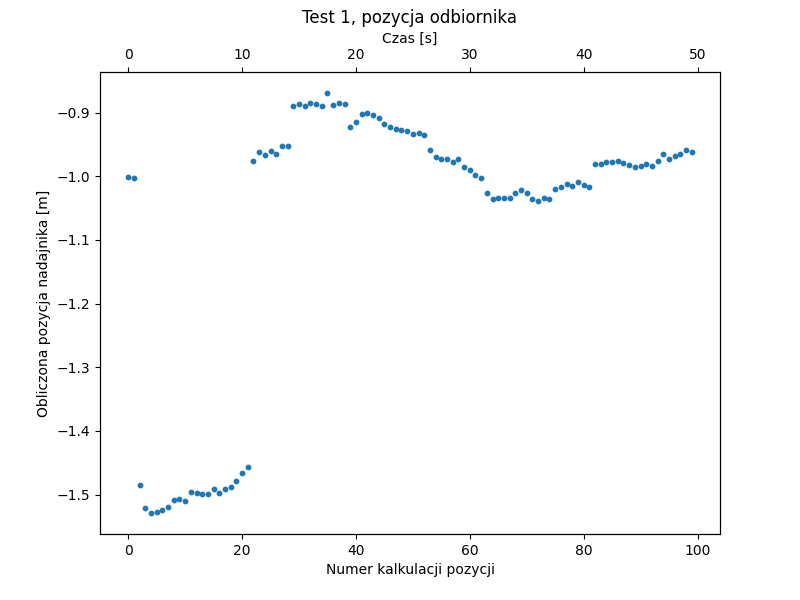
\includegraphics[width=\linewidth]{pics/position/position_1.png}
        \caption{Test 2.}
    \end{subfigure}
\end{figure}
\begin{figure}[H]
    \ContinuedFloat\centering
    \begin{subfigure}{\textwidth}\label{fig:position_2}
        \centering
        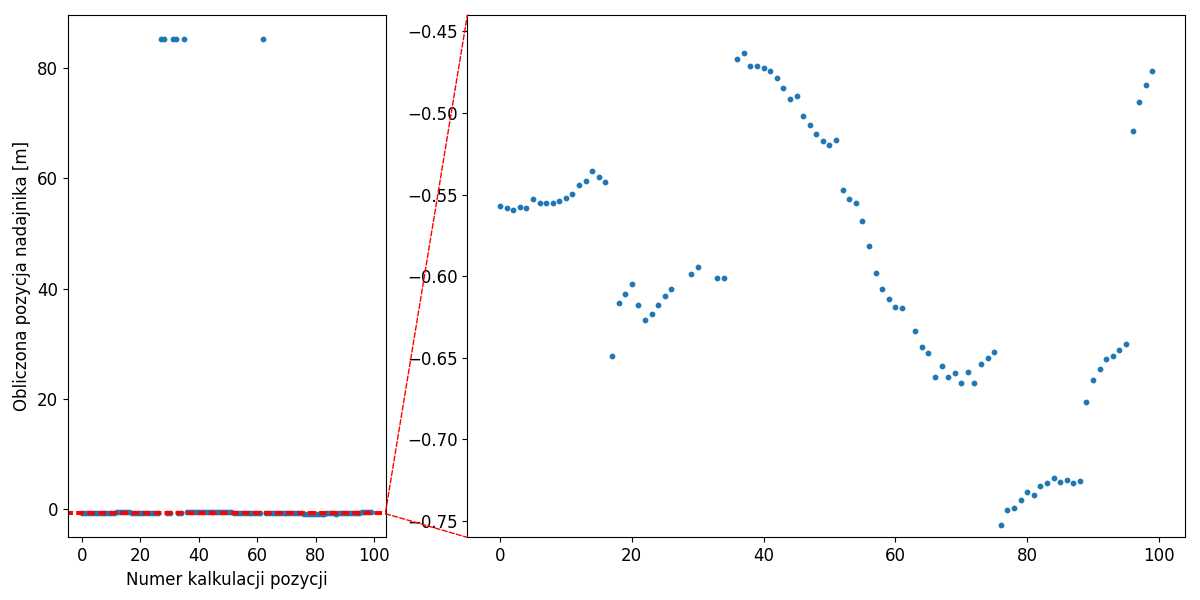
\includegraphics[width=\linewidth]{pics/position/position_2.png}
        \caption{Test 3. Diagram po prawej stanowi powiększenie zaznaczonego obszaru diagramu po lewej.}
    \end{subfigure}
\end{figure}
\begin{figure}[H]
    \ContinuedFloat\centering
    \begin{subfigure}{\textwidth}\label{fig:position_3}
        \centering
        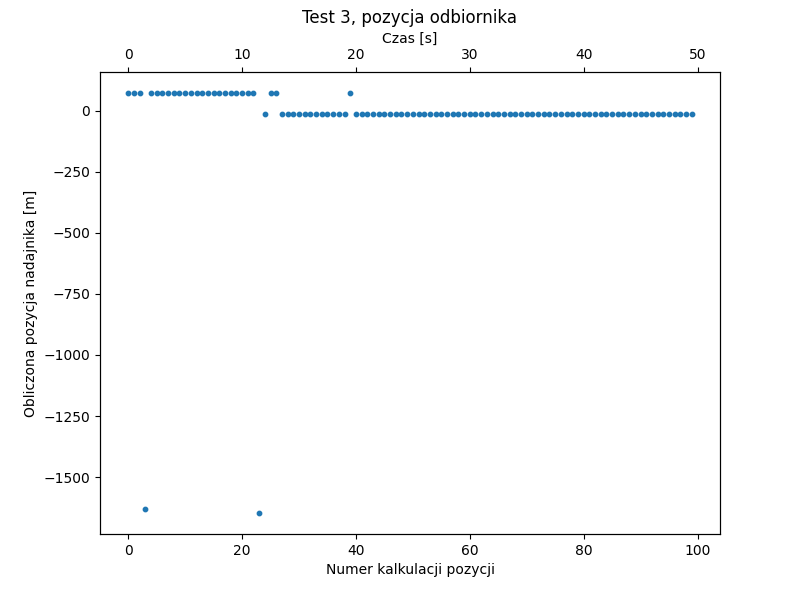
\includegraphics[width=\linewidth]{pics/position/position_3.png}
        \caption{Test 4. Diagramy po prawej stanowią powiększenie odpowiednich obszarów diagramu po lewej.}
    \end{subfigure}
\end{figure}
\begin{figure}[H]
    \ContinuedFloat\centering
    \begin{subfigure}{\textwidth}\label{fig:position_4}
        \centering
        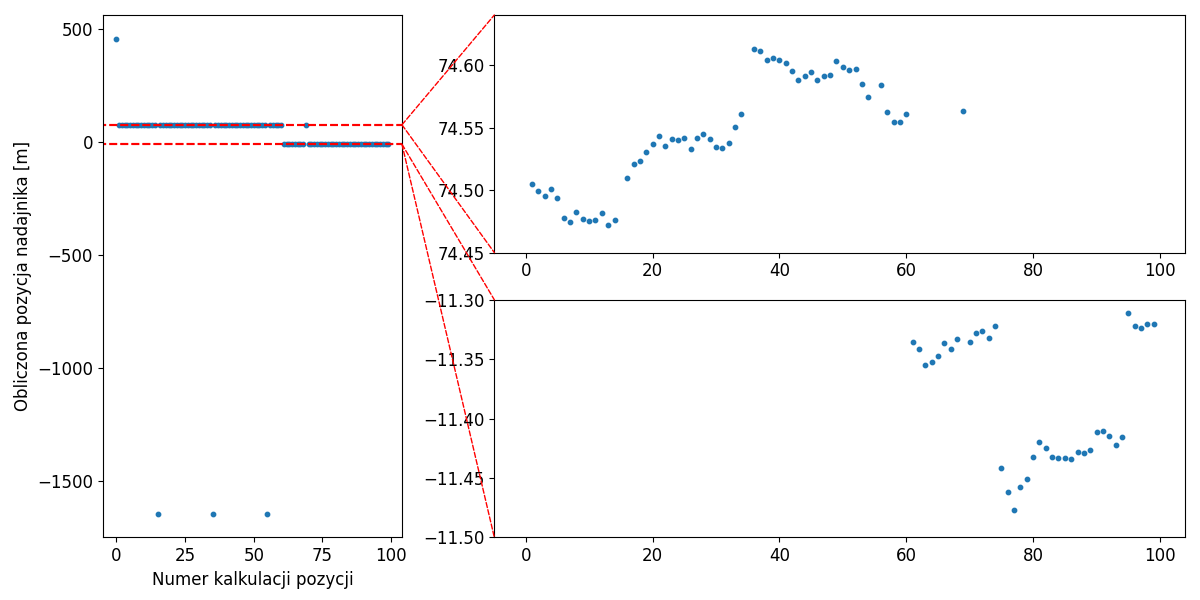
\includegraphics[width=\linewidth]{pics/position/position_4.png}
        \caption{Test 5. Diagramy po prawej stanowią powiększenie odpowiednich obszarów diagramu po lewej.}
    \end{subfigure}
    \caption{Wykres obliczonej pozycji odbiornika w zależności od czasu}
    \label{fig:position}
\end{figure}

\section{Interpretacja wyników i wnioski}

Już na pierwszym z wykresów widać, że wartości wyjściowe algorytmu są niestabilne, współrzędna nadajnika wacha się w przedziale $(-0.98, -0.8)$, a także co jakiś czas następują nagłe przeskoki między następującymi po sobie wartościami. Coraz większa rozbieżność następuje wraz z upływem czasu. Już w drugim teście różnica ekstremalnych odchyleń jest większa niż odległość między nadajnikami, a dokładność jest absolutnie niezadowalająca. Kolejne testy jedynie utwierdzają te obserwacje.

Na niską dokładność i stabilność wyników może mieć wpływ wiele czynników takich jak:

\begin{itemize}
    \item niepoprawna synchronizacja zegarów węzłów,
    \item niepoprawna kalibracja czułości mikrofonów,
    \item fałszywe odczyty wynikające z odbić fali dźwiękowej,
    \item niska jakość rozwiązania aproksymacyjnego.
\end{itemize}

Obserwując skoki pomiędzy sąsiadującymi obserwacjami położenia rozdzielającymi okresy względnej stabilności i mając na uwadze statyczność otoczenia systemu możemy śmiało wysnuć wniosek, że tak nagła zmiana średniej obliczanej wartości może wynikać najprawdopodobniej z błędnej synchronizacji czasu. Wygląda na to, że sygnał wysyłany przez serwer obliczeniowy nie jest odbierany we wszystkich węzłach równocześnie. Następny rozdział będzie poświęcony badaniu i tworzeniu algorytmu synchronizacji zegarów w węzłach.